%!TEX root=../main.tex
\chapter{System Setup}
\label{apdx:setup}
This chapter will go into depth of the Climbing Mont Blanc system and setup information. The goal of this chapter is to complement the setup and handover instructions given by Follan and Støa \cite{mt:T&S}. Section \ref{sec:folder} proposes a uniform code folder structure in the CMB system, introduced by Follan and Støa on the development and production servers of CMB. The purpose is to allow for quicker setup of the system for local development, but also to quickly setup a new development or production server. Sections \ref{sec:fsetup}, \ref{sec:ssetup}, and \ref{sec:bsetup} explain the setup of the frontend, server, and backend respectively for both a new CMB instance and local development. The sections focus is on summarizing, complementing and gathering some of the setup and handover information written by Follan and Støa \cite{mt:T&S}. This will hopefully provide a complete and quick reference documentation of the CMB setup for new developers.

\section{Folder Structure}
\label{sec:folder}
The folder structure for the frontend- and server-code should be equal to the folder structure at development and production servers of CMB. It is recommended to keep the folder structure when developing locally. Having identical folder structures might reduce confusion and bugs that comes up when developing code, as some environment variables in the system depends upon the folder structure. It is much easier to set up the system as well, as little modification is needed to the configuration files to make the system work locally. The setup information is also much easier explained with a uniform folder structure. The proposed folder structure is shown in Figure \ref{fig:workspace}. When explaining the setup information, it is assumed that the folder containing the directories in Figure \ref{fig:workspace} is called \textit{cmb}. \\

The folder structure equals the folder structure at the CMB development and production server. On a CMB development or production server the folder \textit{cmb\_board} would not be present, as this folder contains the code for the CMB backend and would instead be present on the backend board. The folder structure for the frontend, server and backend code are all shown in Figure \ref{fig:folder-structure}. As mentioned, the code is available at Bitbucket via git, and the folder structure should be easy to setup after repository access is granted. The reader is hereby warned that a different folder structure changes the setup information. An overview of the result of the set up of local, development and production CMB system is shown in Figure \ref{fig:setup-overview}. Note that the backend setup is equal in each environment, and is therefore not included in the figure.

\begin{figure}
    \centering
    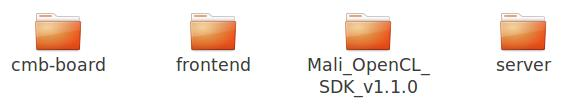
\includegraphics[width=0.8\textwidth, height=0.2\textwidth]{figs/workspace.jpg}
    \caption[]{Workspace folder structure}
    \label{fig:workspace}
\end{figure}

\begin{figure}
    \centering
    \begin{subfigure}[b]{0.2\textwidth}
        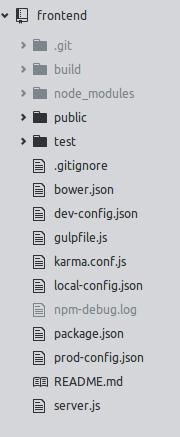
\includegraphics[width=\textwidth]{figs/frontend.jpg}
        \caption{Frontend}
        \label{fig:folders-frontend}
    \end{subfigure}
    ~ %add desired spacing between images, e. g. ~, \quad, \qquad, \hfill etc.
      %(or a blank line to force the subfigure onto a new line)
    \begin{subfigure}[b]{0.2\textwidth}
        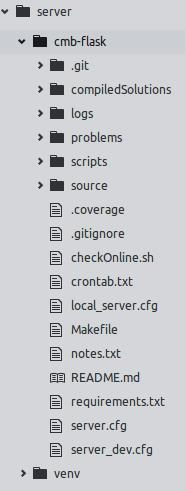
\includegraphics[width=\textwidth]{figs/server.jpg}
        \caption{Server}
        \label{fig:folders-server}
    \end{subfigure}
    ~ %add desired spacing between images, e. g. ~, \quad, \qquad, \hfill etc.
    %(or a blank line to force the subfigure onto a new line)
    \begin{subfigure}[b]{0.2\textwidth}
        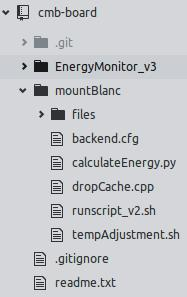
\includegraphics[width=\textwidth]{figs/backend.jpg}
        \caption{Backend}
        \label{fig:folders-backend}
    \end{subfigure}
    \caption[]{Folder structure}\label{fig:folder-structure}
\end{figure}

\clearpage

\begin{figure}
    \centering
    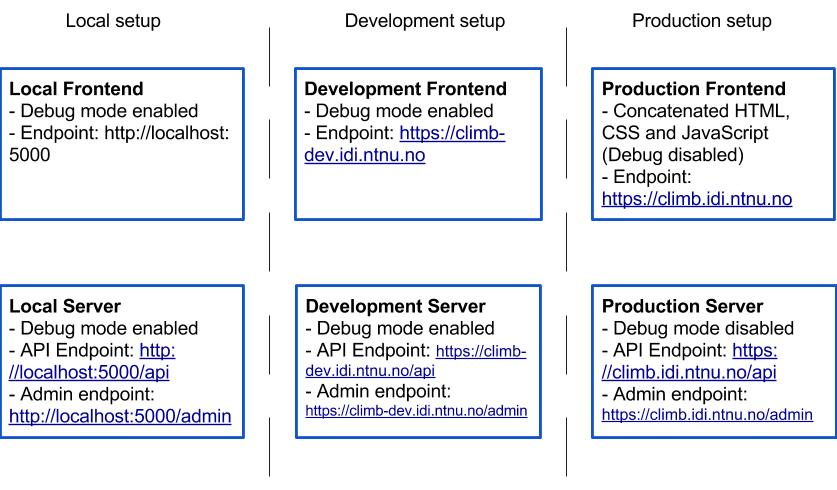
\includegraphics[width=0.9\textwidth, height=0.5\textwidth]{figs/setup-overview.jpg}
    \caption[]{General Overview of the Different Setup Options}
    \label{fig:setup-overview}
\end{figure}

\section{Frontend Setup}
\label{sec:fsetup}
Figure \ref{fig:folders-frontend} shows the structure of the frontend code, and will be relevant in this section. Acquire the frontend code and create the folder structure shown in figure \ref{fig:folders-frontend} before starting setup. This section gathers the setup and handover information from the master thesis of Follan and Støa \cite{mt:T&S}, and is rewritten according to the proposed folder structure to make the setup easier.

\paragraph*{CMB Frontend Setup} \hfill \\
To build the frontend run the following command in the \textit{frontend/} directory:
\begin{lstlisting}[language=sh]
npm install
\end{lstlisting}
The command will install all the required packages with \texttt{npm} \cite{NPM}. The required packages is listed in a file called \textit{package.json}. After running the command, the required packages will be saved in a folder called \textit{node\_modules}. To build the system as it is used on the production server, the build tool \texttt{gulp} \cite{GULP} is used with the following command in the \textit{frontend/} directory:
\begin{lstlisting}[language=sh]
gulp prod
\end{lstlisting}
The command will concatenate the HTML, CSS and JavaScript files which makes the code more efficient, and lowers the number of requests made when fetching data to the browser. However, since this concatenation reduces the number of source files, the code will be harder to debug. After running the commands, the frontend should be available at the URL \url{https://climb.idi.ntnu.no}, but keep in mind that it will not function properly before the server has been set up. The frontend will assume that a server API is available at \url{https://climb.idi.ntnu.no/api} to fetch data, which requires a running server as explained in section \ref{sec:ssetup}. To build the development version instead, stay in the \textit{frontend/} directory and run:
\begin{lstlisting}[language=sh]
gulp dev
\end{lstlisting}
The command will not concatenate the HTML, CSS and JavaScript files, which will make it easier to debug using developer tools in the browser. The frontend should now be available at \url{https://climb-dev.idi.ntnu.no}. The development frontend also requires a running server with an API available at \url{https://climb-dev.idi.ntnu.no/api}, as explained in section \ref{sec:ssetup}.

\paragraph*{Local Setup} \hfill \\
First, as above, run the following command in the \textit{frontend/} directory:
\begin{lstlisting}[language=sh]
npm install
\end{lstlisting}
The command will install all dependencies from listed in \textit{package.json}.
\noindent
To build the frontend for local development, run the following command in the \textit{frontend/} directory:
\begin{lstlisting}
gulp
\end{lstlisting}
The command will build the project as it is done on the development server, but the website is instead available at \url{http://localhost:5000}. This means that a local version of the server should also be run (described in \Cref{sec:ssetup}). The command will also watch for changes in the code, and for every change it will run the unit tests and rebuild the code. All gulp tasks are defined in the \textit{gulpfile.js}, and new tasks can be added there. New code or modifications to existing code should be done in the \textit{public/} folder.

\paragraph*{Unit Tests and Linter} \hfill \\
To make the unit tests run correctly, all \texttt{bower} \cite{BOWER} dependencies must be installed. This is done by running the following command in the \textit{frontend/} directory:
\begin{lstlisting}[language=sh]
bower install
\end{lstlisting}
This will install all dependencies from the \textit{bower.json} file in the bower components folder. To run the tests, enter the \textit{frontend/} directory and run the tests through the \textit{gulp} task:
\begin{lstlisting}
gulp test
\end{lstlisting}
When the tests are run, a directory called \textit{coverage/} is automatically created within the \textit{frontend/} directory. This directory contains an HTML report of the test run.\\

To run the \texttt{jshint} \cite{JSHINT} linter manually, run the following \textit{gulp task} in the \textit{frontend/} directory:
\begin{lstlisting}[language=sh]
gulp jshint
\end{lstlisting}
The command will report linter errors if any.

\section{Server Setup}
\label{sec:ssetup}
The directory structure for the server can be seen in Figure \ref{fig:folders-server}. Acquire the server code and create the folder structure in Figure \ref{fig:folders-server} before starting setup. The paragraphs "Installation and Configuration", "Database Setup and Migration" and "Unit Tests and Linter" are setup information created by Follan and Støa. The paragraphs are rewritten and complemented using the proposed folder structure to make the setup process easier.

\paragraph*{Virtual Environment and Dependencies} \hfill \\
A Python Virtual Environment (VE) \cite{VIRTUALENV} should be installed and used when developing and running the server code. When installed, create a new VE by running the following command in the \textit{server/} directory:
\begin{lstlisting}[language=sh]
virtualenv venv
\end{lstlisting}
The command will create the folder structure \textit{venv/} within the \textit{server/} directory. One need to activate the VE to install packages and use the packages installed within it. The Unix command \textit{source} is used to activate the VE. An example from the \textit{server/} directory is:
\begin{lstlisting}[language=sh]
source ./venv/bin/activate
\end{lstlisting}

To install all required packages needed on the server, activate the VE and use \texttt{pip} \cite{PIP} to install the required packages within the VE. All required packages is listed in the \textit{requirements.txt} file, and is installed by running the following command from the \textit{server/cmb-server/} directory:
\begin{lstlisting}[language=sh]
pip install -r requirements.txt
\end{lstlisting}
The above command will install all required Python dependencies needed for correct execution of the server. Installation of requirements needs to be done both when developing locally and when setting up a new CMB server. \\

To deactivate the VE, execute the following command anywhere:
\begin{lstlisting}[language=sh]
deactivate
\end{lstlisting}

\paragraph*{Installation and Configuration} \hfill \\
To correctly compile the uploaded solutions on the server, a \textit{Mali OpenCL SDK} \cite{MALI} library is needed. It is recommended to install it as shown in Figure \ref{fig:workspace}. It is also a requirement to create a directory called \textit{workspace/} within the extracted folder of the Mali OpenCL SDK. The CMB server also needs OpenMP 4.0, gcc-4.9 and g++-4.9 to compile the uploaded programs correctly. The following steps installs the required compilers and libraries:
\begin{lstlisting}
sudo apt-get-repository ppa:ubuntu-toolchain-r/test
sudo apt-get update
sudo apt-get install gcc-4.9 g++-4.9
sudo apt-get install build-essential
\end{lstlisting}

Uncomplicated Firewall (UFW) \cite{UFW} and Fail2Ban \cite{F2B} are installed and configured by running the commands below:
\begin{lstlisting}
sudo apt-get install fail2ban
sudo ufw allow 80
sudo ufw allow 443
sudo ufw enable
\end{lstlisting}
UFW should already be present, and does not need installation. The second and third command above allows requests to port 80 and 443. That is, all HTTP and HTTPS request should be allowed to pass to the server. Fail2Ban should work out of the box.\\

Nginx \cite{NGINX} can be installed in the following manner:
\begin{lstlisting}
sudo apt-get update
sudo apt-get install nginx
\end{lstlisting}

Some environment variables need to be set up to configure a CMB server correctly. Firstly, the Unix environment variable \textit{APPLICATIONS\_SETTINGS} need to be set. This environment variable points to a file that contains application specific variables, depending on if the server is either a production, development or a local server. The files \textit{server.cfg}, \textit{server\_dev.cfg} and \textit{local\_server.cfg} present in the directory \textit{server/cmb-flask/} represents the application settings for a production, development or a local server respectively. For example, the IP address of a backend board, the path for the Mali OpenCL SDK, the database URI and the server port is all present in the configuration files among other variables. \Cref{sec:server-cfg} gives an example of how the file \textit{local\_server.cfg} might look like. It is very important to enter these values correctly. \\

The next environment variables that need to be set are \textit{CMB\_MAIL\_USERNAME}, \textit{CMB\_MAIL\_PASSWORD}, \textit{CMB\_SECRET\_KEY} and \textit{CMB\_TOKEN\_SECRET}. The variables \textit{CMB\_MAIL\_USERNAME} and \textit{CMB\_MAIL\_PASSWORD} are used to send an email to the CMB administrators when an error occurs, which is crucial if setting up a production environment. The variables \textit{CMB\_SECRET\_KEY} and \textit{CMB\_TOKEN\_SECRET} are used for session token generation, authenticating messages and more.  When developing locally, these variables can stay unchanged and can be copied from the file \textit{local\_server.sh} present in the directory \textit{cmb-flask/scripts/}. If setting up a development or production server, contact the CMB team, and they will provide the information to set these variables correctly. It is recommended to enter the variables into \textit{\$HOME/.bash\_profile} or some similar file that loads the environment variables when starting up a new shell. \\

The environment variable \textit{SLQALCHEMY\_DATABASE\_URI}\footnote{The database URI describes which database to connect to. Example with MySQL: mysql://$<$username$>$:$<$password$>$@$<$host$>$/$<$db\_name$>$.} and \textit{SERVER\_TIMEOUT} also needs to be set in the \textit{\$HOME/.bash\_profile} or some similar file which loads the environment variables. The server timeout describes the timeout of SSH commands and is currently defined to be 95 seconds. \\

Run the following command from the directory \textit{server/cmb-flask/scripts/} to start either a development or production server:
\begin{lstlisting}
./init_cmb start
\end{lstlisting}
The command will start the whole CMB system, including the frontend and \textit{push.py}. Keep in mind that the system will not function correctly before a backend has been set up, as described in section \ref{sec:bsetup}. The above command also allows the arguments \textit{stop} and \textit{restart} as well, to stop or restart the CMB system respectively. The above command is the recommended way of starting either a production or development server. To start a local server, run the following command in the \textit{server/cmb-flask/source/} directory:
\begin{lstlisting}
python server.py start
\end{lstlisting}
This will start the server without \textit{Gunicorn} \cite{GUNICORN}. Running the server without Gunicorn makes it easier to debug, as only a single instance of the server is running. However, it is possible to launch the CMB locally with the \textit{init\_cmb} script locally as well if wanted. No matter the method of running the server, it will create a callable API at endpoint \url{https://localhost:5000}. It is important to initialize the database (see below) before running the server the first time. \\

The following lines can also be added in the file \textit{/etc/rc.local} to make automatically start the system when booting the server:
\begin{lstlisting}
su climber -s /bin/bash -l -c
    "/srv/climber/cmb/server/cmb-flask/scripts/init\_cmb.sh start" >
    /dev/null
\end{lstlisting}

\paragraph*{Database Setup and Migration} \hfill \\
To clear and initialize a database for a new server, run the following command in the directory \textit{server/cmb-flask/}:
\begin{lstlisting}
python init_db.py
\end{lstlisting}
If there is a modification to the database models (read table schema), one needs to \textit{migrate} \footnote{Migration is the task of updating or reverting a database schema while trying to preserve the data that might be present in the database.} the database. Migration happens by creating a migration script, generated by running the following command in from the \textit{server/cmb-flask/source/} directory:
\begin{lstlisting}
python server.py db migrate -m "some message."
\end{lstlisting}
This will create a new directory within \textit{server/cmb-flask/source/} called \textit{migrations} if not present, with the auto generated migrations script within. To launch the migration script and alter the database table schema, stay in the directory \textit{server/cmb-flask/source/} and run:
\begin{lstlisting}
python server.py db upgrade
\end{lstlisting}
On the production and development servers, this is done automatically through Jenkins when there is a change to the database tables. The migration script is also added to the git repository so that the above step can be executed manually. \\

The production and development databases are provided by the IDI department \cite{IDI}. If developing locally, remember that MySQL needs to be installed and a local database needs to be set up. Remember to set the correct database URI in the \textit{\$HOME/.bash\_profile} or similar file as described above.

\paragraph*{Unit Tests and Linter} \hfill \\
After installing and activating the virtual environment above, make sure all required packages from \textit{requirements.txt} are installed. From the directory \textit{server/cmb-flask/source/}, run the following command:
\begin{lstlisting}
nosetests --with-coverage --cover-package=admin,routes,cmb_utils,server,database tests/*.py
\end{lstlisting}
This will run automatic unit tests with \texttt{nose} \cite{NOSE} for all tests present in the directory \textit{server/cmb-flask/source}. It will also generate a cover report, with an extensive overview of the code covered by the tests. If developing a new test, it might be useful running just a single test. To run a single test, execute the following command the \textit{server/cmb-flask/source/} folder:
\begin{lstlisting}
nosetest tests/problems_test.py
\end{lstlisting}
This will run the tests present in the \textit{problems\_test.py} file. One can simply run another test set by changing the file name to another file present in the \textit{server/cmb-flask/source/tests/} directory. \\
\noindent
To run the \textit{flake8} linter, stay in the \textit{server/cmb-flask/source/} directory and run:
\begin{lstlisting}
flake8 .
\end{lstlisting}
The terminal window will report potential errors.

\section{Backend Setup}
\label{sec:bsetup}
This section explains the setup of a new Odroid-XU3 board with the folder structure equal to the one in Figure \ref{fig:folders-backend}. The folder structure is relevant when setting up the CMB board code as explained below. The paragraph ``CMB Setup'' contains instructions and information made by Follan and Støa, which is further complemented (uninstalling \textit{lightdm} \cite{m:lightdm}) and rewritten to make setup easier.

\paragraph*{Odroid-XU3 Setup} \hfill \\
A new Odroid-XU3 board should have a fresh installation of Xubuntu installed available at the Odroid website \cite{m:odroid}. The Xubuntu installation information given here is inspired by the information stated at the Odroid website \cite{m:odroid-i}. The Odroid-XU3 can either boot from a MicroSD card or a special module called eMMC module. The eMMC module needs to be connected to a eMMC module reader as seen in the Figure \ref{fig:emmc} to be able to flash. A Unix operating system is assumed used when flashing the OS image onto an eMMC module or a MicroSD. For flashing of OS images onto MicroSD like media using Windows, refer to the Odroid website \cite{m:odroid}. After downloading a new Operating System image, flash the connected MicroSD card or eMMC module with the following commands within the folder where the image is downloaded:
\begin{lstlisting}
unxz some-xubuntu-image-file.img.xz
sudo dd if=/dev/zero of=</dev/path/of/card> bs=4M conv=fsync
sudo dd if=<some-xubuntu-image-file.img> of=</dev/path/of/card> bs=4M conv=fsync
sync
\end{lstlisting}
The path of the MicroSD card or eMMC module can be found by monitoring the directory \textit{/dev/} before and after connecting the device. The connected device will appear as sdX, where X is some alphabetical character. As mentioned, CMB uses the EnergyMonitor program to measure energy consumption, and it is important to check that the downloaded OS image supports the EnergyMonitor program.\\

\begin{figure}
    \centering
    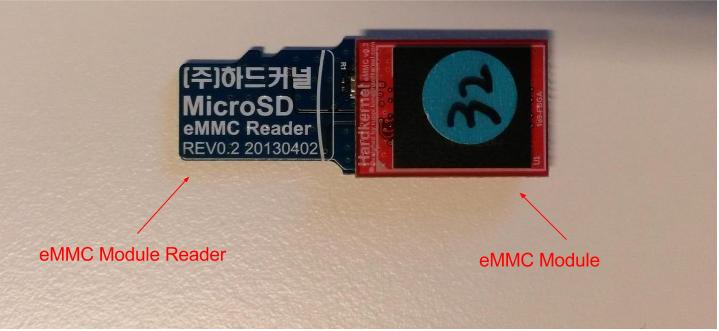
\includegraphics[width=0.9\textwidth, height=0.4\textwidth]{figs/emmc.jpg}
    \caption[]{eMMC Module and Reader}
    \label{fig:emmc}
\end{figure}

\noindent
After installing the OS, connect either the MicroSD or eMMC module to the board\footnote{Check out \url{http://odroid.com/dokuwiki/doku.php?id=en:xu3_bootmode_configuration} on how to toggle between booting from eMMC module and MicroSD.}. Then boot and connect the Odroid-XU3 to a monitor either trough mini-HDMI or a DisplayPort. An automatic login will happen to a user called \textit{odroid}. Open a terminal window and create two more users by running the following commands:
\begin{lstlisting}
useradd climber
passwd climber
useradd worker
\end{lstlisting}
This creates two users, \textit{climber} and \textit{worker}. When prompted for a password for the \textit{climber} user, enter the password given to you by the CMB team. These two users are needed to execute commands and run programs through the server. Additionally, enter the following line to the end of the file \textit{sudoers} located in the directory \textit{/etc/}:
\begin{lstlisting}
...
climber    ALL=(worker) NOPASSWD: ALL
...
\end{lstlisting}
The line will make sure that the \textit{worker} user have the privileges to execute the uploaded programs. The command \textit{visodu} should be used to add the line to the \textit{sudoers} file. \\

The backend should install OpenSSH and OpenSSH Server if not already installed \cite{m:openssh}. The two services can be installed and configured to CMB by executing the following commands:
\begin{lstlisting}
sudo apt-get install ssh-client
sudo apt-get install ssh-server
ssh-keygen -t rsa
ssh-copy-id username@ip-to-server
\end{lstlisting}
When prompted for something, just hit enter. After executing the commands above, login to the board can happen without entering a password. This will make sure that the server does not get prompted for a password when it needs to execute scripts at the backend. You should not be prompted for a password when logging into the board from the server after executing these commands. \\

Uncomplicated Firewall (UFW) and Fail2Ban are installed much the same way as on the server. Execute the following commands to install and configure both services:
\begin{lstlisting}
sudo apt-get install fail2ban
sudo ufw allow from 127.241.0.0/16
sudo ufw enable
\end{lstlisting}
The board should not be accessible from outside the NTNU network, which this UFW configuration ensures.

\paragraph*{CMB Setup} \hfill \\
Follan and Støa reported the CMB backend setup in their Master thesis \cite{mt:T&S}. The commands to setup the CMB backend code are repeated here, and extended with the removal of \textit{lightdm} \cite{m:lightdm}. Log in as \textit{climber} at the board through SSH and fetch the backend code from Bitbucket (clone the repository with git), and run the following commands to correctly setup the CMB backend: \\

\begin{lstlisting}
# Link binary
sudo ln -sf /lib/ld-linux-armhf.so.3 /lib/ld-linux.so.3
# programs and packages used by runscript_v2.sh, EnergyMonitor and
calculateEnergy.py.
sudo apt-get install python-scipy time qt4-default libqwt-dev
# install g++ and gcc 4.9 to support OpenMP 4.0
sudo add-apt-repository ppa:ubuntu-toolchain-r/test
sudo apt-get update
sudo apt-get install gcc-4.9 g++-4.9
sudo apt-get install build-essential
# add following line to /etc/rc.local. This script is run automatically on boot,
# and is needed for tempAdjustment to read current temperature.
# Permissions are reset when rebooting.
chmod +r /sys/devices/10060000.tmu/temp
# These are needed by the EnergyMonitor_v3.
# Make sure executable name is "EnergyMonitor"
cd cmb-board/EnergyMonitor_v3
qmake
make
# Remove lightdm for accurate energy readings
sudo apt-get purge lightdm
# compile dropCache.cpp to dropCache and make it an auxiliary executable.
# dropCache is responsible for clearing the cache before running a program.
cd ~/cmb-board/mountBlanc
g++ -O2 dropCache.cpp -o dropCache
chmod 4710 dropCache
\end{lstlisting}
Download the Mali OpenCL SDK v1.1 and copy the folders \textit{common}, \textit{lib} and \textit{include} into the directory \textit{cmb-board}. The folders can also be transferred from the server.

\section{Local Server Configuration File}
\label{sec:server-cfg}
The configuration file presented here assumes that the project have been structured as proposed in section \ref{sec:folder}. An example configuration file is listed below, which only requires one to find the path to the \textit{cmb/} directory and the executing backend IP address.

\begin{lstlisting}[language=sh]
SERVER_PORT=5000
BOARD_IP="THE_BOARD_IP_ADDRESS"
MALI_DIR="<path-to-cmb>/cmb/Mali_OpenCL_SDK_v1.1.0"
FLASK_DIR="<path-to-cmb>/cmb/server/cmb-flask/"
FRONTEND_DIR="<path-to-cmb>/cmb/frontend/"
UPLOAD_FOLDER="<path-to-cmb>/cmb/server/cmb-flask/problems"
MAIL_SERVER='smtp.gmail.com'
MAIL_PORT=465
MAIL_USE_TLS=False
MAIL_USE_SSL=True
GUNICORN_LOG_LEVEL="debug"
VERSION="dev"
\end{lstlisting}
